\documentclass[aspectratio=169]{beamer}
\usetheme{Madrid}
\usecolortheme{default}
\usepackage{booktabs,amsmath}
\graphicspath{{figs/}}
\title[EXEC\_13]{EXEC\_13: Fixed-Scale $t_N$ Analysis (EJ-204)}
\subtitle{Gerardo's request --- meeting 12 Jun 2026}
\author{Ren\'e R\'ios}
\institute{Universidad de La Serena (ULS)}
\date{2026-06-13}
\begin{document}
\begin{frame}\titlepage\end{frame}

\begin{frame}
\frametitle{F1 — Overlay $t_{4}$, normalised (fixed scale)}
\centering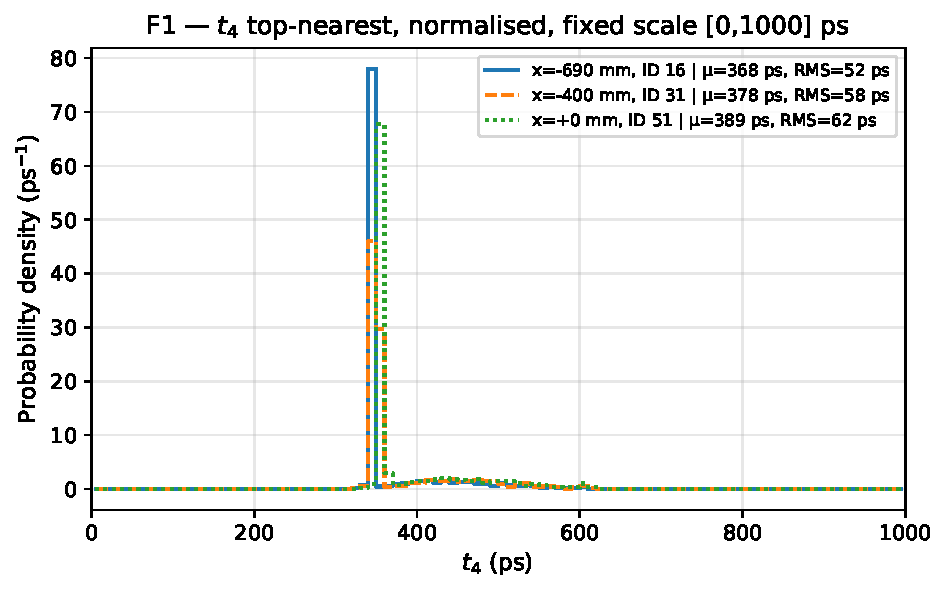
\includegraphics[width=0.82\textwidth]{exec13_f1_t4pe_overlay_norm}
\begin{block}{\footnotesize How to read this plot}
\scriptsize\textbf{Why:} EXEC\_12 histograms used auto-scale; this re-bins at 10\,ps with fixed [0,1000]\,ps range so run shapes are visually comparable.\quad\textbf{Axes:} x: $t_{4}$ arrival time (ps); y: probability density (norm) or events/10\,ps (abs).\quad\textbf{Takeaway:} Narrow, nearly Gaussian distribution; RMS dominated by order-stat fluctuations.
\end{block}

\end{frame}

\begin{frame}
\frametitle{F1 — Overlay $t_{4}$, absolute counts (fixed scale)}
\centering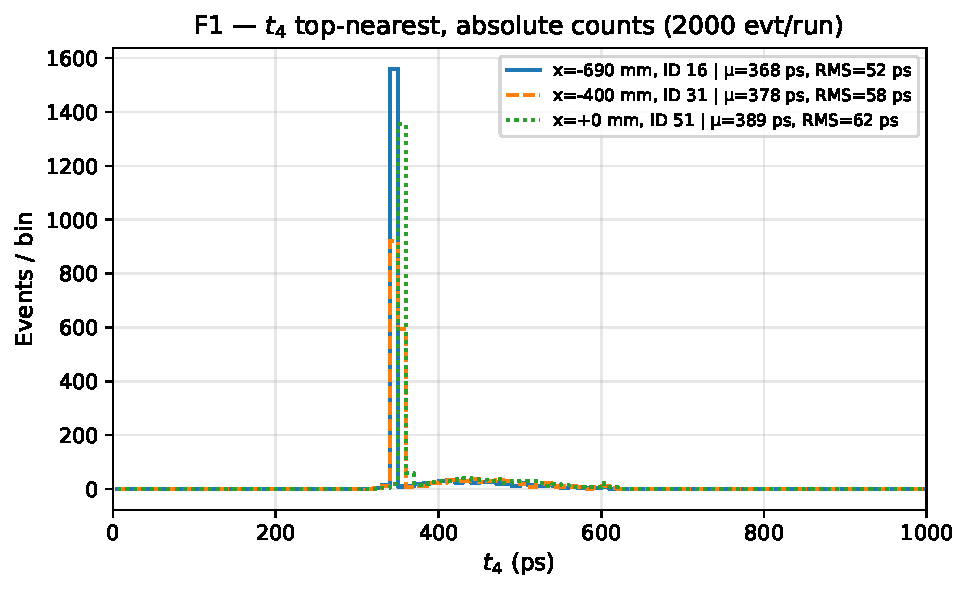
\includegraphics[width=0.82\textwidth]{exec13_f1_t4pe_overlay_abs}
\begin{block}{\footnotesize How to read this plot}
\scriptsize\textbf{Why:} EXEC\_12 histograms used auto-scale; this re-bins at 10\,ps with fixed [0,1000]\,ps range so run shapes are visually comparable.\quad\textbf{Axes:} x: $t_{4}$ arrival time (ps); y: probability density (norm) or events/10\,ps (abs).\quad\textbf{Takeaway:} Narrow, nearly Gaussian distribution; RMS dominated by order-stat fluctuations.
\end{block}

\end{frame}

\begin{frame}
\frametitle{F1 — Individual panels $t_{4}$ (identical scale)}
\centering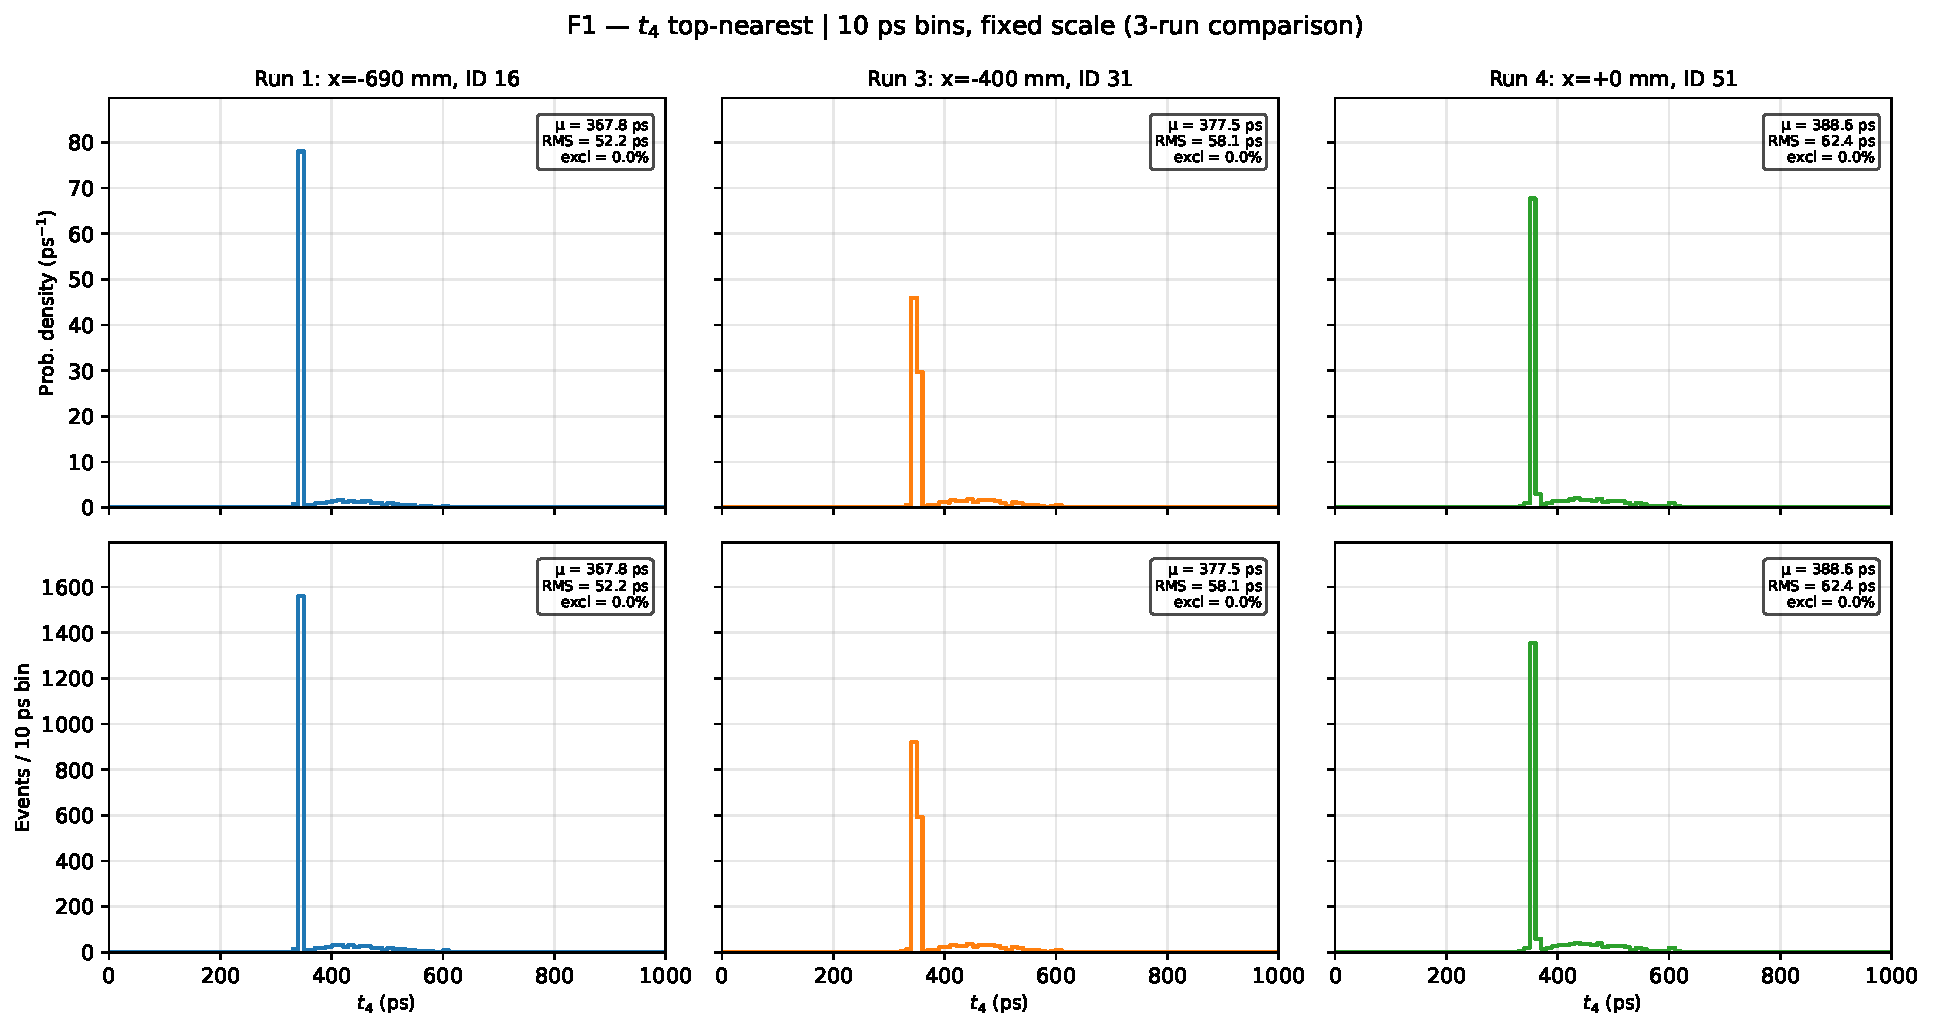
\includegraphics[width=0.95\textwidth]{exec13_f1_t4pe_panels}
\begin{block}{\footnotesize How to read this plot}
\scriptsize\textbf{Why:} EXEC\_12 histograms used auto-scale; this re-bins at 10\,ps with fixed [0,1000]\,ps range so run shapes are visually comparable.\quad\textbf{Axes:} x: $t_{4}$ arrival time (ps); y: probability density (norm) or events/10\,ps (abs).\quad\textbf{Takeaway:} Narrow, nearly Gaussian distribution; RMS dominated by order-stat fluctuations.
\end{block}

\end{frame}

\begin{frame}
\frametitle{F1 — Overlay $t_{20}$, normalised (fixed scale)}
\centering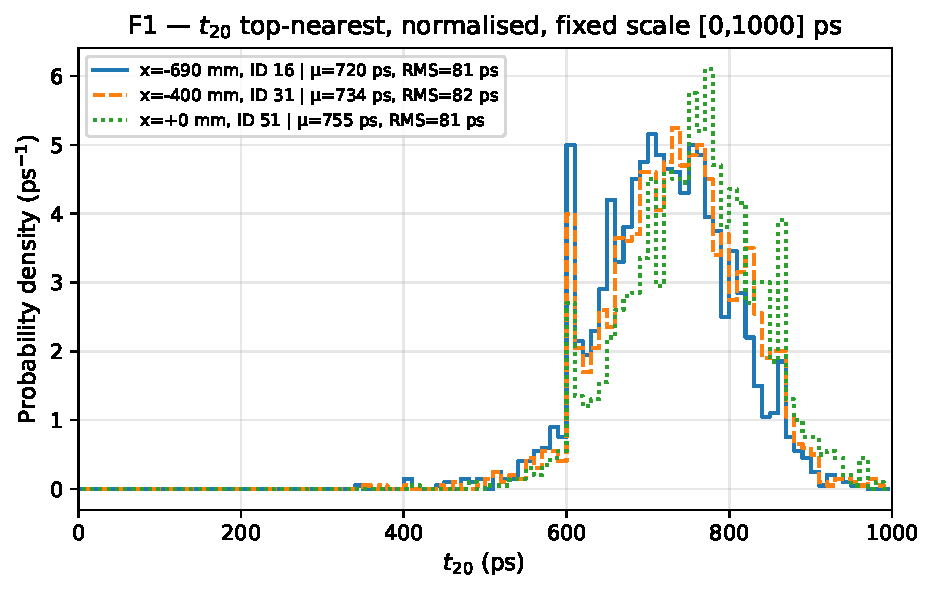
\includegraphics[width=0.8\textwidth]{exec13_f1_t20pe_overlay_norm}
\begin{block}{\footnotesize How to read this plot}
\scriptsize\textbf{Why:} EXEC\_12 histograms used auto-scale; this re-bins at 10\,ps with fixed [0,1000]\,ps range so run shapes are visually comparable.\quad\textbf{Axes:} x: $t_{20}$ arrival time (ps); y: probability density (norm) or events/10\,ps (abs).\quad\textbf{Takeaway:} Broader, skewed distribution; shape dominated by Landau $N_{{pe}}$ spread.
\end{block}

\end{frame}

\begin{frame}
\frametitle{F1 — Overlay $t_{20}$, absolute counts (fixed scale)}
\centering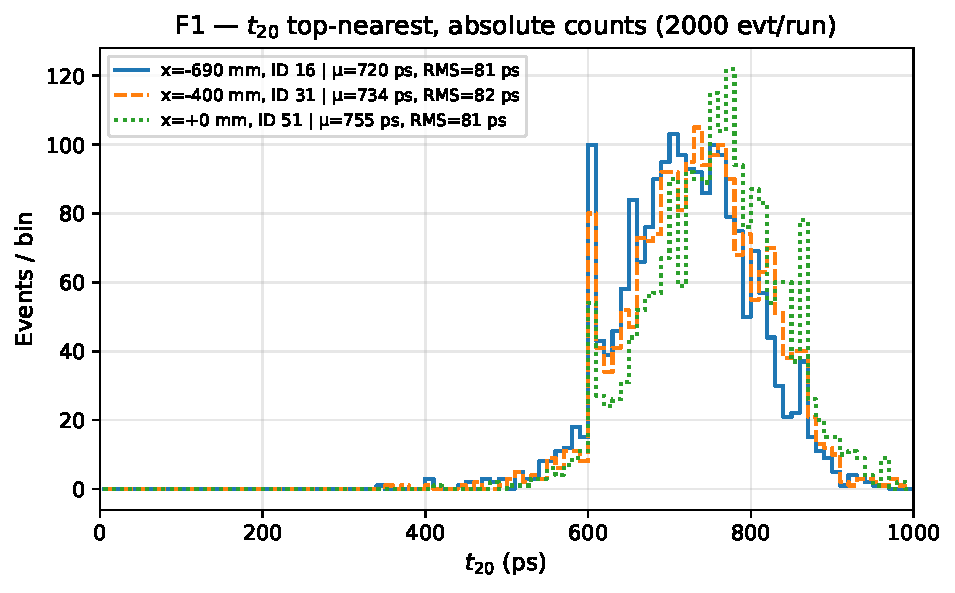
\includegraphics[width=0.8\textwidth]{exec13_f1_t20pe_overlay_abs}
\begin{block}{\footnotesize How to read this plot}
\scriptsize\textbf{Why:} EXEC\_12 histograms used auto-scale; this re-bins at 10\,ps with fixed [0,1000]\,ps range so run shapes are visually comparable.\quad\textbf{Axes:} x: $t_{20}$ arrival time (ps); y: probability density (norm) or events/10\,ps (abs).\quad\textbf{Takeaway:} Broader, skewed distribution; shape dominated by Landau $N_{{pe}}$ spread.
\end{block}

\end{frame}

\begin{frame}
\frametitle{F1 — Individual panels $t_{20}$ (identical scale)}
\centering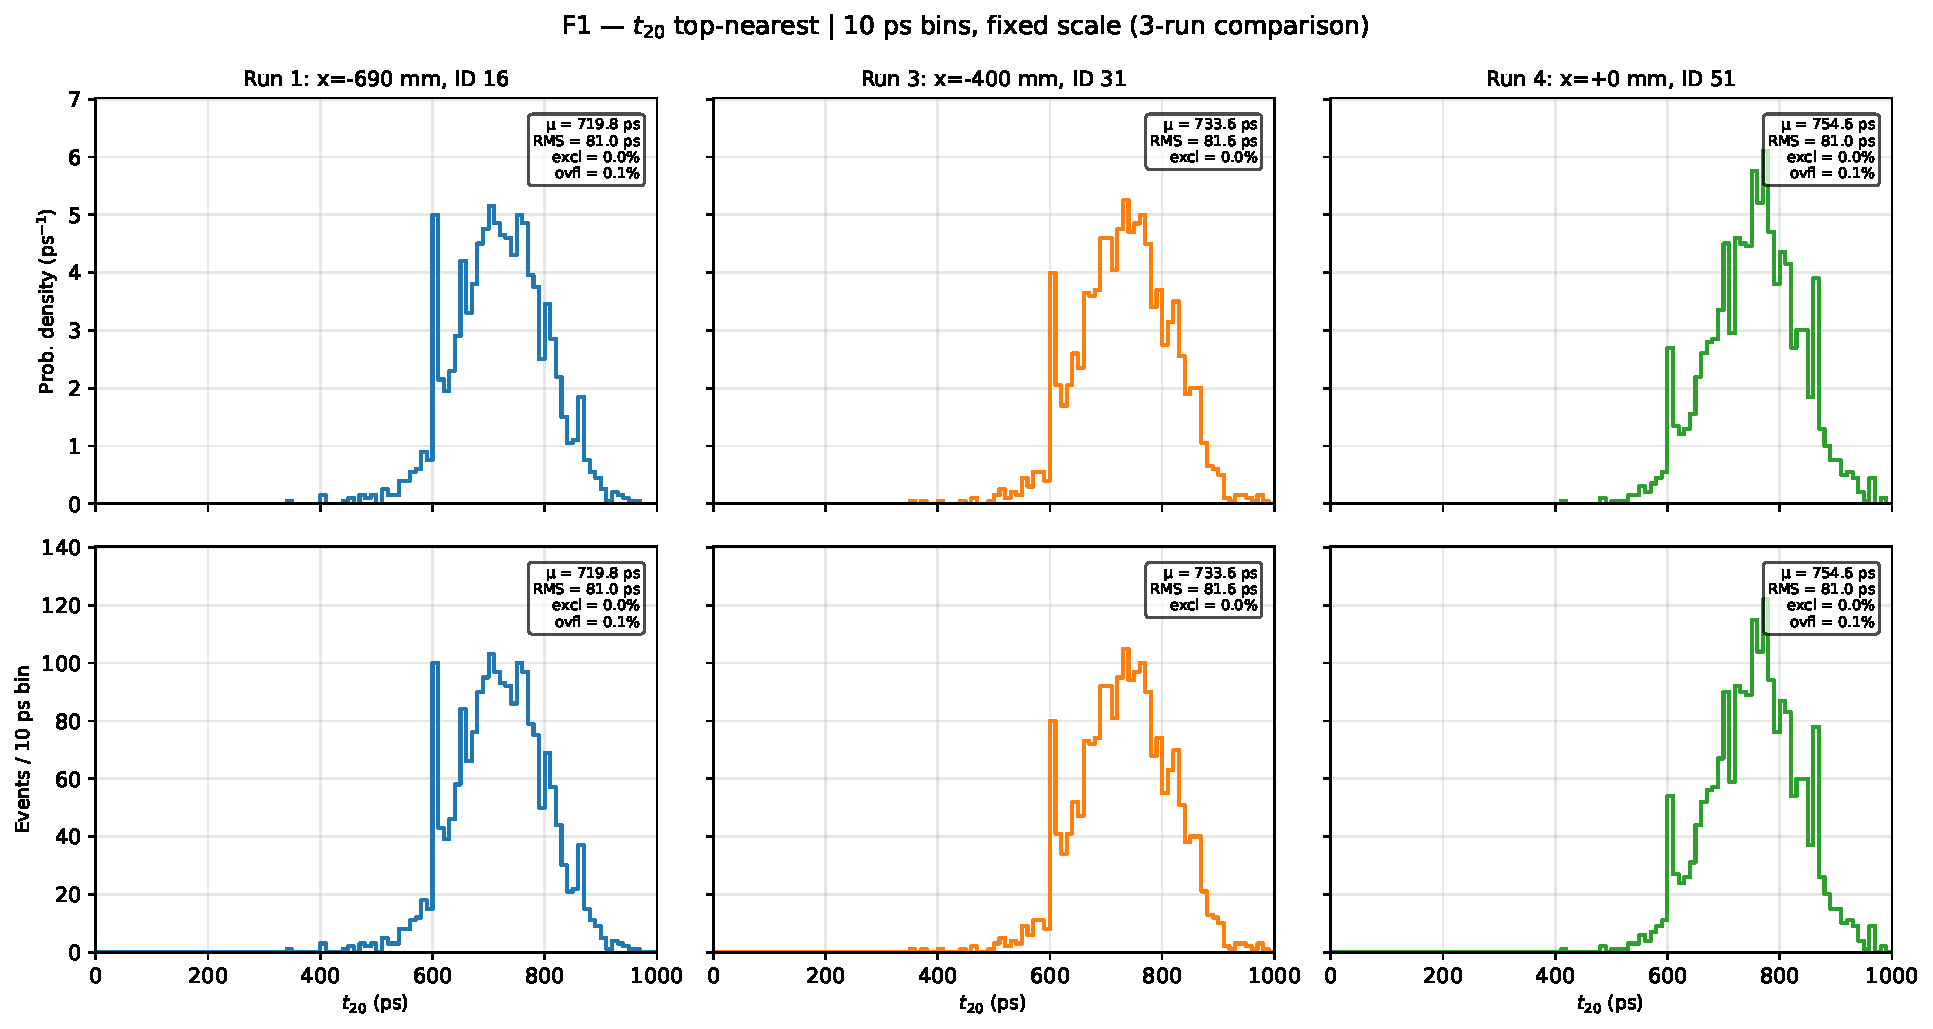
\includegraphics[width=0.95\textwidth]{exec13_f1_t20pe_panels}
\begin{block}{\footnotesize How to read this plot}
\scriptsize\textbf{Why:} EXEC\_12 histograms used auto-scale; this re-bins at 10\,ps with fixed [0,1000]\,ps range so run shapes are visually comparable.\quad\textbf{Axes:} x: $t_{20}$ arrival time (ps); y: probability density (norm) or events/10\,ps (abs).\quad\textbf{Takeaway:} Broader, skewed distribution; shape dominated by Landau $N_{{pe}}$ spread.
\end{block}

\end{frame}

\begin{frame}
\frametitle{F2 — Run 1: $x=-690$\,mm cluster dispersion}
\centering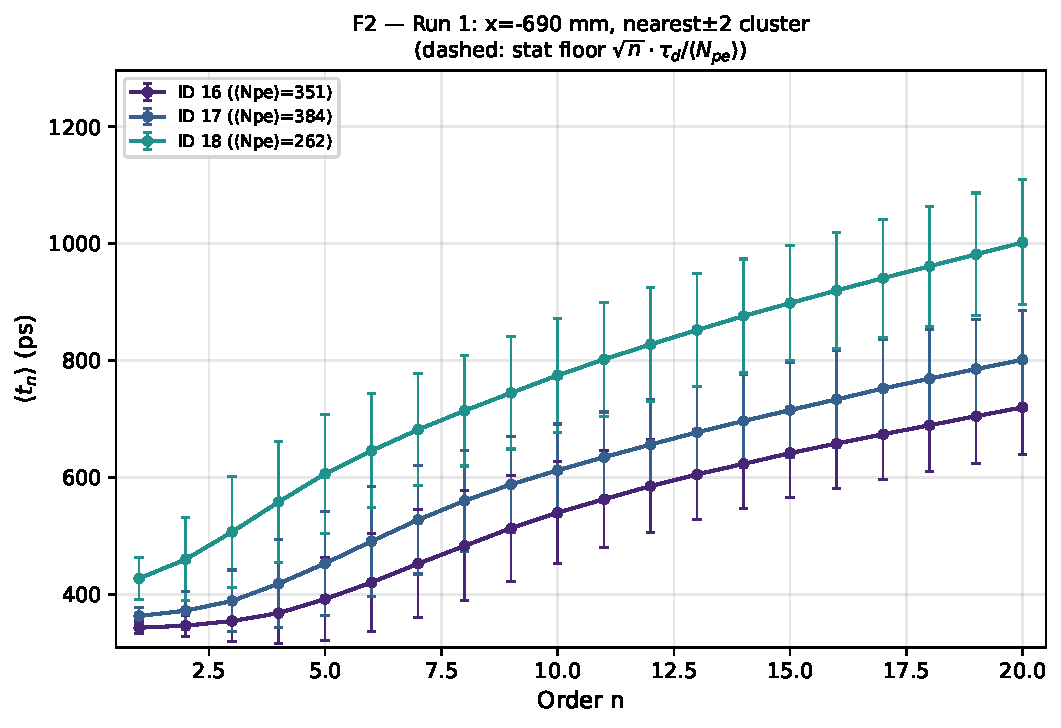
\includegraphics[width=0.72\textwidth]{exec13_f2_cluster_-690mm}
\begin{block}{\footnotesize How to read this plot}
\scriptsize\textbf{Why:} Gerardo's clustering question: do neighbour SiPMs $\pm1,\pm2$ carry the same timing as the nearest?\quad\textbf{Axes:} x: photon order $n$; y: $\langle t_n\rangle$ (ps). Error bars = RMS. Dashed: stat floor $\sqrt{n}\tau_d/\langle N_{pe}\rangle$.\quad\textbf{Takeaway:} Neighbours approach stat floor faster when their $\langle N_{pe}\rangle$ is comparable to the nearest; far neighbours are dominated by stat noise → can be dropped.
\end{block}

\end{frame}

\begin{frame}
\frametitle{F2 — Run 3: $x=-400$\,mm cluster dispersion}
\centering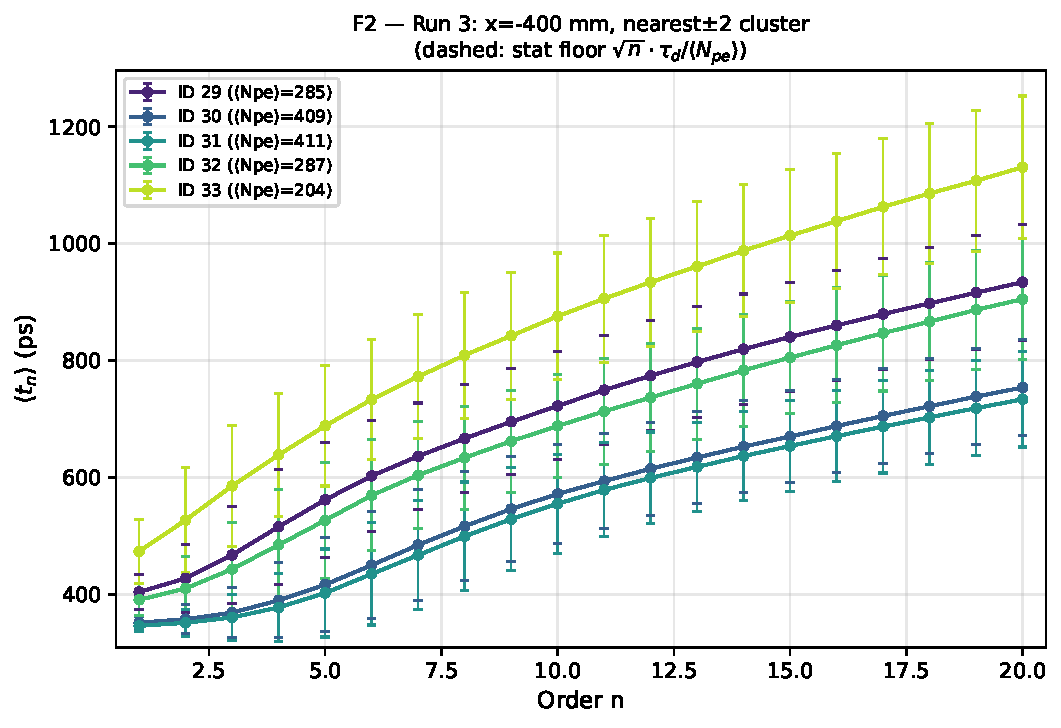
\includegraphics[width=0.72\textwidth]{exec13_f2_cluster_-400mm}
\begin{block}{\footnotesize How to read this plot}
\scriptsize\textbf{Why:} Gerardo's clustering question: do neighbour SiPMs $\pm1,\pm2$ carry the same timing as the nearest?\quad\textbf{Axes:} x: photon order $n$; y: $\langle t_n\rangle$ (ps). Error bars = RMS. Dashed: stat floor $\sqrt{n}\tau_d/\langle N_{pe}\rangle$.\quad\textbf{Takeaway:} Neighbours approach stat floor faster when their $\langle N_{pe}\rangle$ is comparable to the nearest; far neighbours are dominated by stat noise → can be dropped.
\end{block}

\end{frame}

\begin{frame}
\frametitle{F2 — Run 4: $x=+0$\,mm cluster dispersion}
\centering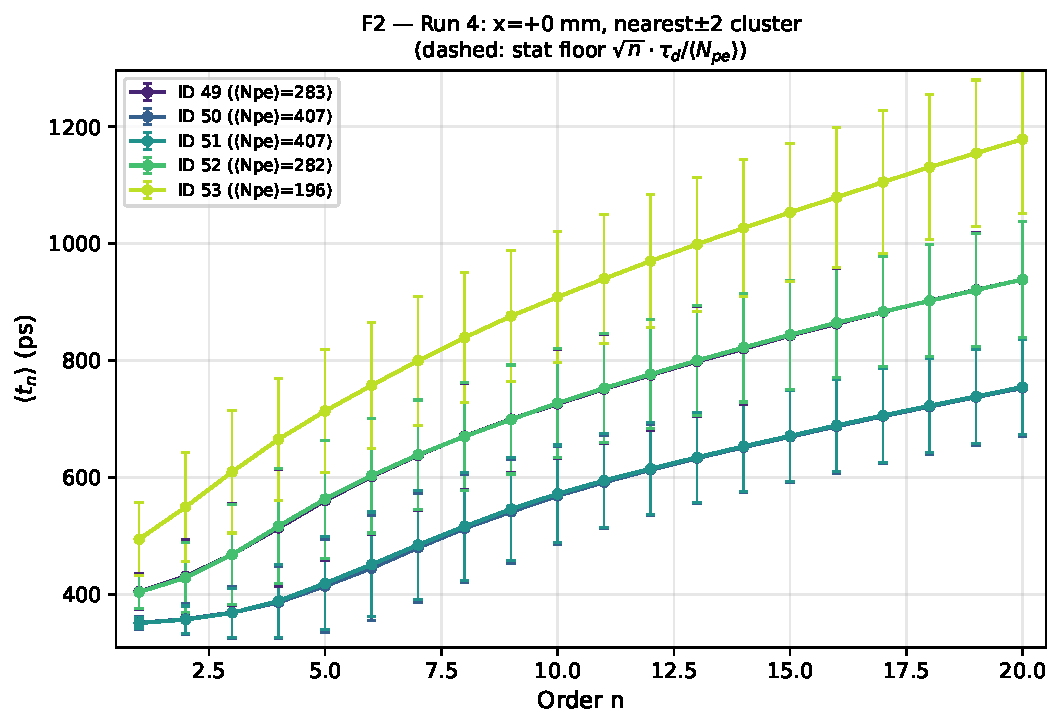
\includegraphics[width=0.72\textwidth]{exec13_f2_cluster_+0mm}
\begin{block}{\footnotesize How to read this plot}
\scriptsize\textbf{Why:} Gerardo's clustering question: do neighbour SiPMs $\pm1,\pm2$ carry the same timing as the nearest?\quad\textbf{Axes:} x: photon order $n$; y: $\langle t_n\rangle$ (ps). Error bars = RMS. Dashed: stat floor $\sqrt{n}\tau_d/\langle N_{pe}\rangle$.\quad\textbf{Takeaway:} Neighbours approach stat floor faster when their $\langle N_{pe}\rangle$ is comparable to the nearest; far neighbours are dominated by stat noise → can be dropped.
\end{block}

\end{frame}

\begin{frame}
\frametitle{F3 — Top $N_{pe}$ profile (all 70 channels, fixed scale)}
\centering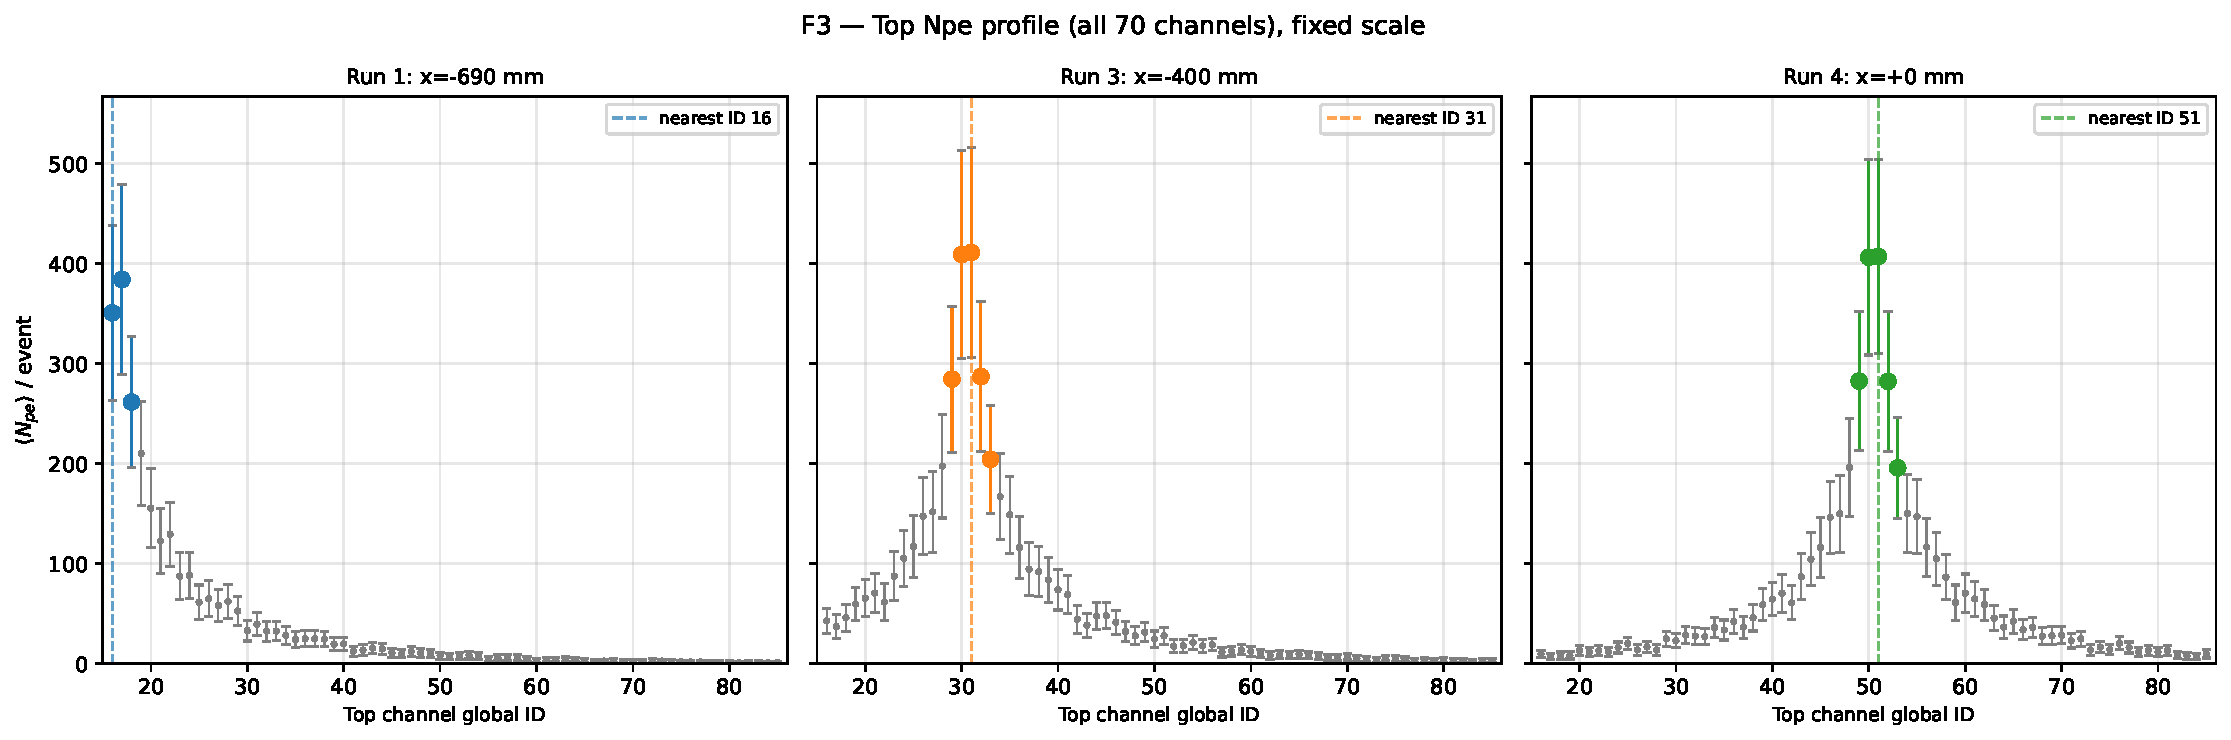
\includegraphics[width=0.98\textwidth]{exec13_f3_npe_profile}
\begin{block}{\footnotesize How to read this plot}
\scriptsize\textbf{Why:} Verify that the nearest channel is correctly identified as the Npe maximum; shows photon budget across the full top array.\quad\textbf{Axes:} x: global channel ID (16--85); y: $\langle N_{pe}\rangle$/event $\pm$ RMS. Highlighted: cluster $\pm$2.\quad\textbf{Takeaway:} Npe falls off rapidly away from the track; $\pm$2 neighbours still collect useful light.
\end{block}

\end{frame}

\begin{frame}
\frametitle{F4 — Timing profile $\langle t_{4}\rangle$ (eff$\geq$0.99, fixed scale)}
\centering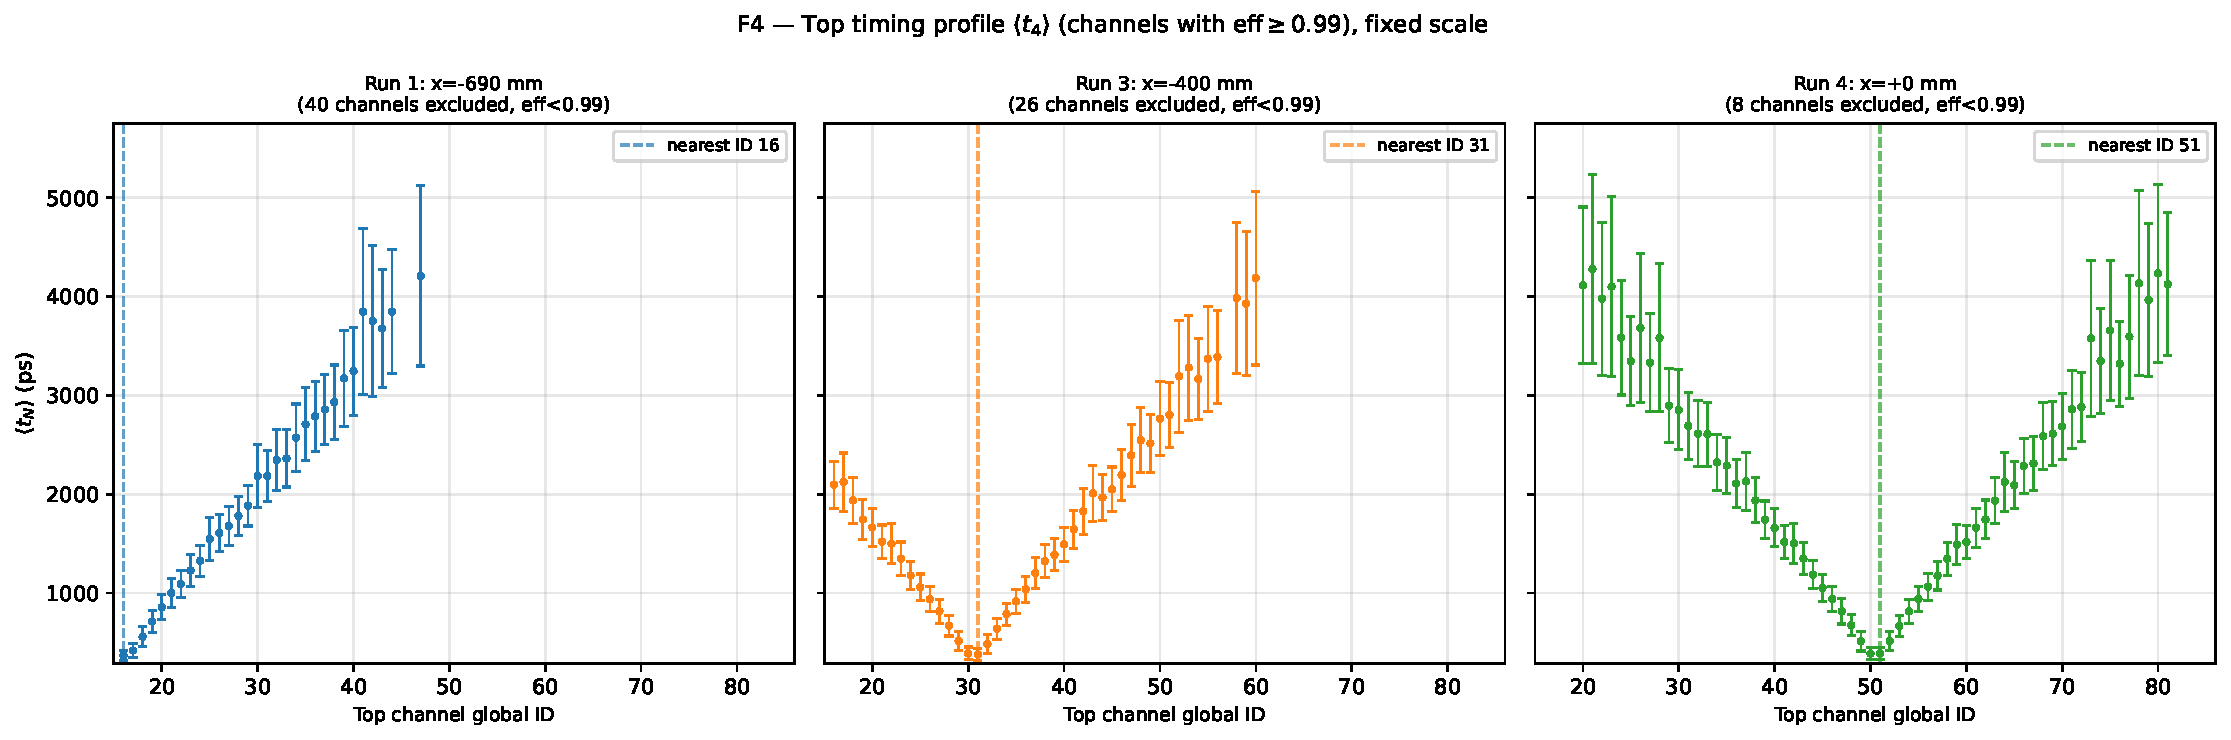
\includegraphics[width=0.98\textwidth]{exec13_f4_timing_t4pe}
\begin{block}{\footnotesize How to read this plot}
\scriptsize\textbf{Why:} Only channels with efficiency $\geq0.99$ are shown; far-end channels that never reach threshold are excluded and listed in exec13\_f4\_timing\_profile.csv.\quad\textbf{Axes:} x: global channel ID; y: $\langle t_N\rangle$ (ps) $\pm$ RMS.\quad\textbf{Takeaway:} Timing rises steeply for channels far from the track (longer optical path + lower $N_{pe}$).
\end{block}

\end{frame}

\begin{frame}
\frametitle{F4 — Timing profile $\langle t_{20}\rangle$ (eff$\geq$0.99, fixed scale)}
\centering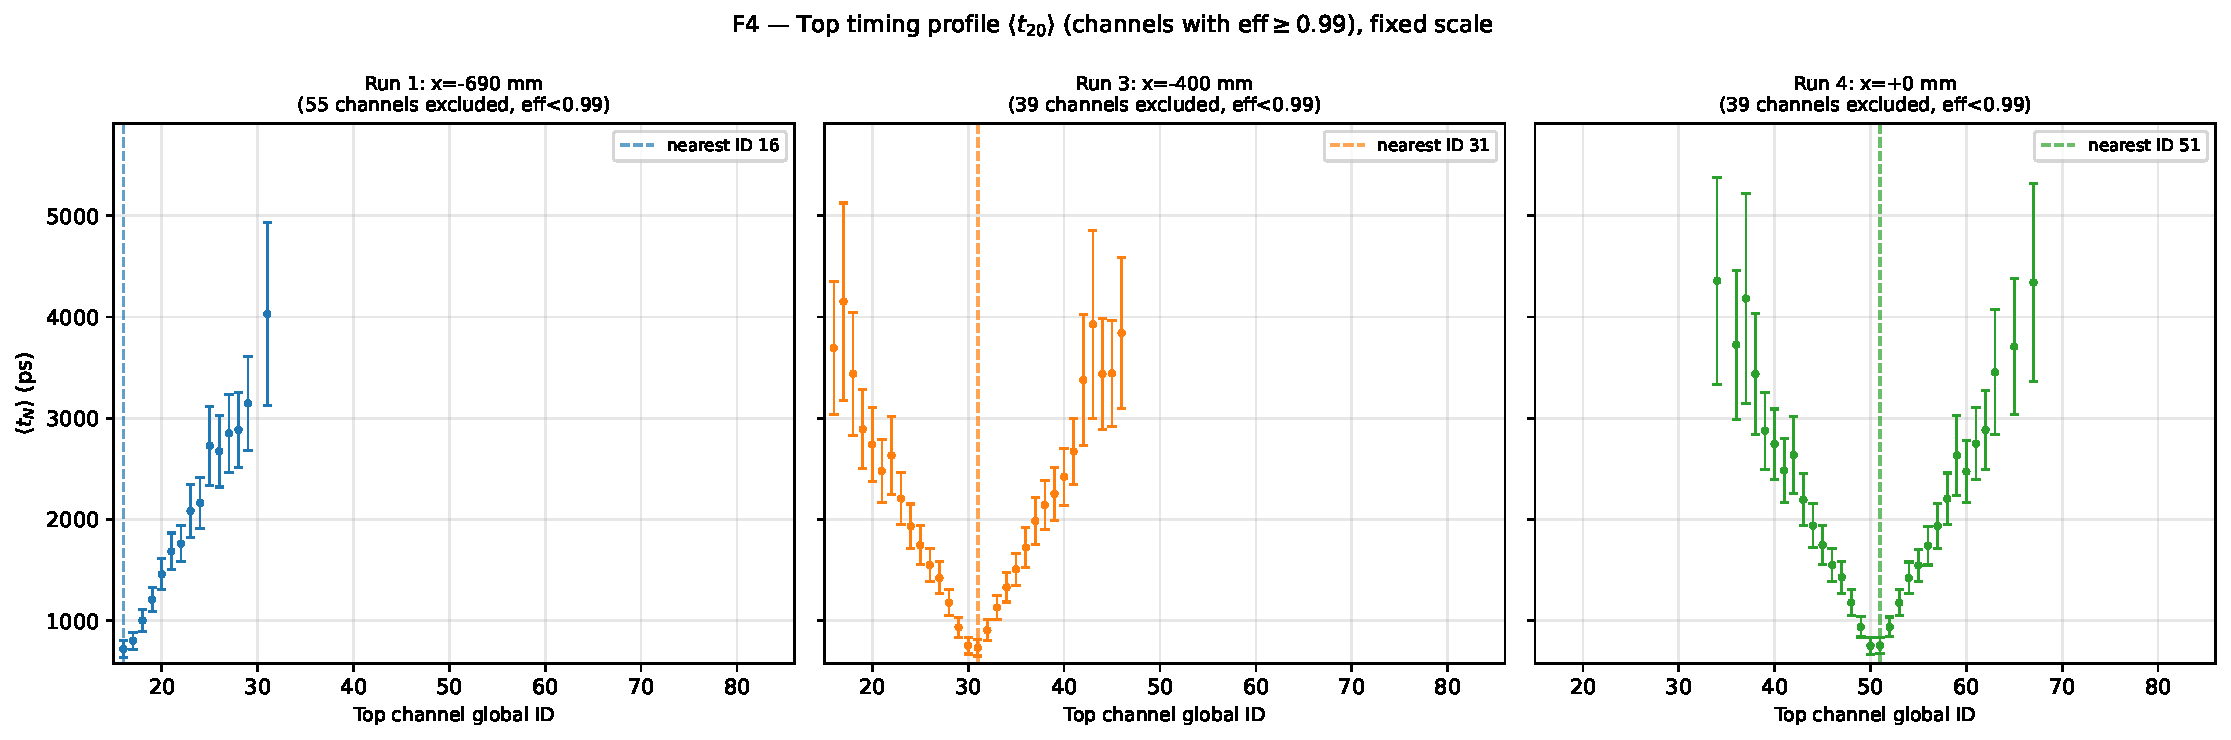
\includegraphics[width=0.98\textwidth]{exec13_f4_timing_t20pe}
\begin{block}{\footnotesize How to read this plot}
\scriptsize\textbf{Why:} Only channels with efficiency $\geq0.99$ are shown; far-end channels that never reach threshold are excluded and listed in exec13\_f4\_timing\_profile.csv.\quad\textbf{Axes:} x: global channel ID; y: $\langle t_N\rangle$ (ps) $\pm$ RMS.\quad\textbf{Takeaway:} Timing rises steeply for channels far from the track (longer optical path + lower $N_{pe}$).
\end{block}

\end{frame}

\begin{frame}
\frametitle{Backup: validation gates}
\small
\begin{itemize}
  \item \textbf{G1}: nearest IDs = \{$-690\to16$, $-400\to31$, $0\to51$\} (EXEC\_12 diagonal) --- must pass before plotting
  \item \textbf{G2}: all figure panels share identical axis limits --- verified programmatically post-plot
  \item \textbf{G3}: $n_{\rm events}=2000$ per run --- verified from ROOT file
  \item \textbf{G4}: $n_{\rm in}+n_{\rm excl}+n_{\rm ovfl}=2000$ per histogram --- bookkeeping check
\end{itemize}
\vspace{4pt}
\scriptsize Gate results: \texttt{exec13\_gates.csv}.
Commit: \texttt{5783a0d2914b}.
Stats table: \texttt{exec13\_f1\_tn\_histograms.csv} (no manual transcription).

\end{frame}


\begin{frame}
\frametitle{Cierre: m\'etodo y procedencia}
\small
\begin{itemize}
  \item \textbf{Generaci\'on:} figuras y CSVs producidos por an\'alisis autom\'atico (Claude Code)
        sobre los ROOT de EXEC\_12 (campa\~na EJ-204, OPSC-101). Sin re-simulaci\'on.
  \item \textbf{Validaci\'on manual pendiente:} R.\ R\'ios verificar\'a en ROOT los valores de
        $\mu$ y RMS de $t_4$/$t_{20}$ del canal nearest (tolerancia $\sim\mathrm{RMS}/\sqrt{2000}$).
        Hasta esa validaci\'on, los valores exhibidos son los del pipeline del agente.
  \item \textbf{Infraestructura de c\'omputo:} simulaciones de EXEC\_12 corridas en el servidor
        t0minidaq (solo detalle log\'istico, no afiliaci\'on).
  \item \textbf{Procedencia de commits:} el slide de gates cita \texttt{5783a0d} (HEAD antes del
        an\'alisis $=$ tag \texttt{pre-exec13-checkpoint}); el commit que genera las figuras y CSVs
        es \texttt{c030e880}. El autoritativo de la fuente de c\'odigo es \texttt{c030e880}; los
        ROOT de datos viven en \texttt{\$DATA\_ROOT} (fuera del repositorio).
\end{itemize}
\end{frame}

\begin{frame}
\frametitle{Cierre: observaciones y temas abiertos}
\small
\begin{itemize}
  \item \textbf{F1 --- sub-resoluci\'on del n\'ucleo de $t_4$:} $\sigma_{\rm fit}(t_4)\approx 8$--9\,ps
        (EXEC\_12); un bin de 10\,ps no resuelve el n\'ucleo. Pendiente: bin $\leq5$\,ps con zoom,
        o ajuste gaussiano al core.
  \item \textbf{F1 --- artefacto de binning:} diferencias de altura de pico en la versi\'on
        normalizada de $t_4$ reflejan en qu\'e borde de bin cae el modo (no anchos f\'isicos
        distintos). Interpretaci\'on cuidadosa requerida.
  \item \textbf{F3 --- efecto window-track en $x=-690$\,mm:} nearest geom\'etrico ID\,16
        ($\langle N_{pe}\rangle=350.9$) colecta menos que ID\,17 ($\langle N_{pe}\rangle=384.2$).
        La diagonal de EXEC\_12 ancla el nearest en ID\,16 (criterio max-$N_{pe}$, que rompe
        el empate geom\'etrico). Efecto window-track documentado; no es un error.
  \item \textbf{F2 --- rango de $n$ verificado:} $n=1\ldots20$ seg\'un script
        (\texttt{TN\_MAX\_ORDER=20}); confirmado leyendo \texttt{exec13\_f2\_cluster\_dispersion.csv}.
        Consistente con lo especificado.
  \item \textbf{Resultado positivo --- $t_{20}$ del nearest:}
        $\mu\approx720/734/755$\,ps, RMS\,$\approx81$\,ps para $x=-690/-400/0$\,mm (valores
        exactos del CSV: 719.8\,/\,733.6\,/\,754.6\,ps). Timing del Top aproximadamente
        independiente de la posici\'on de impacto longitudinal.
\end{itemize}
\end{frame}

\end{document}
